\chapter{基于加密流原始载荷的主机属性发现}

前一章是基于TCP/IP协议栈指纹识别细粒度主机属性地研究,虽然识别效果较好,但这种方法对于特征的提取与构造比较依赖于丰富的网络流量分析经验,导致人工成本和时间成本较高。本章提出了一种基于深度学习模型的主机属性识别技术,利用表示学习的思想,不需要借助任何专家知识,只需将网络流的原始流数据作为分类器输入,便可完成细粒度的主机属性发现,并拥有更佳的识别效果。本章首先从该方法的背景意义和技术路线开始介绍,然后从可视化角度分析原始流信息的特征规律,接着通过分组实验对比不同深度学习模型的适用性,最后分析该方法的实验结果。

\section{引言}

由于近些年来计算性能和数据规模的发展,深度学习模型再度兴起,在信息时代的多个领域都有着重要应用。本章将神经网络模型引入主机属性发现技术中,利用表示学习思想自动挖掘加密流量指纹,用于细粒度主机属性的识别。

如图4.1所示,本方法首先从TLS加密会话中提取TCP SYN包和TLS Clinet Hello包的原始流信息,在经过归一化处理和平整对齐后,传入训练后的深度人工神经网络模型,即可得到客户端主机的多维主机属性。

\begin{figure}[!htbp]
    \centering
    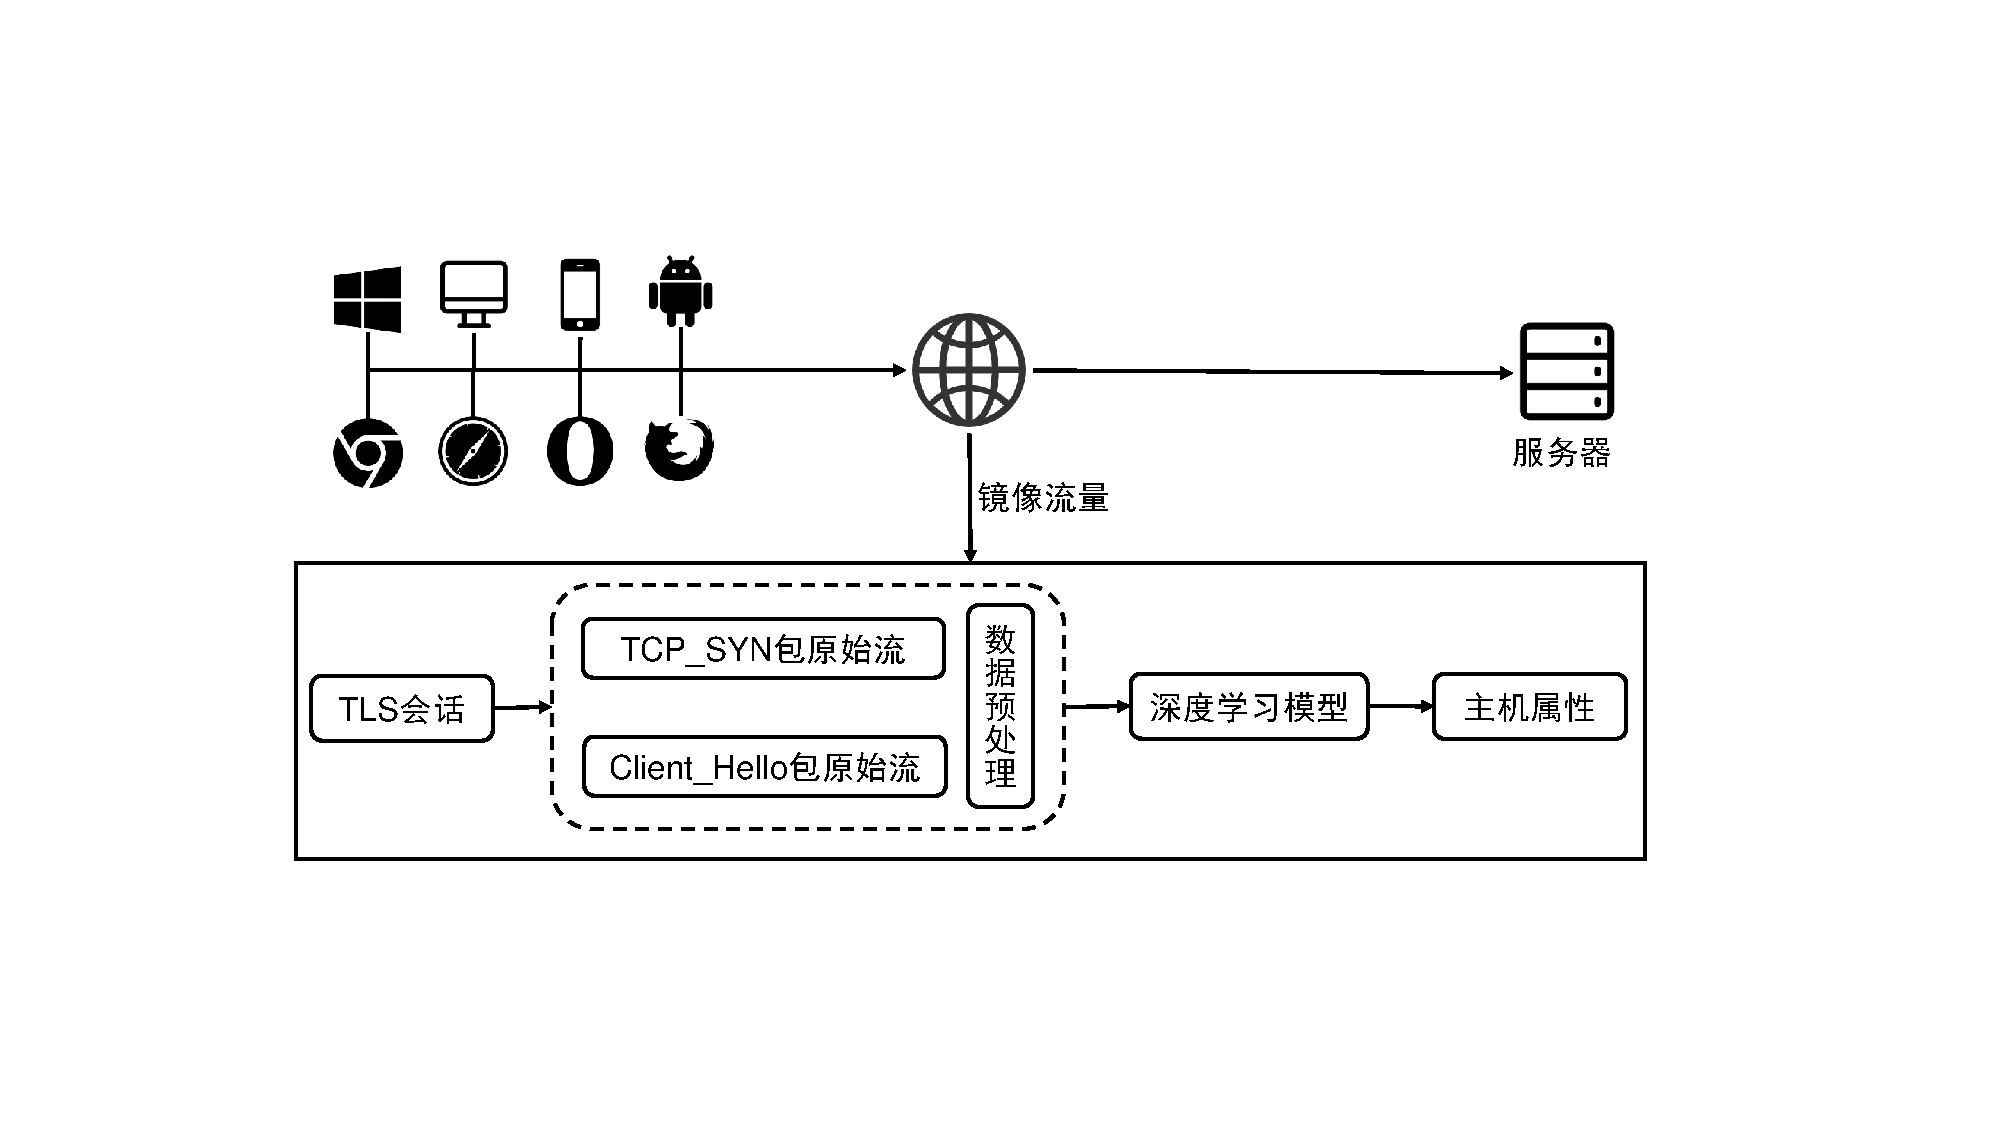
\includegraphics[width=0.9\textwidth]{研究点2结构}
    \bicaption{基于加密流原始载荷的主机属性发现}{Host attribute discovery based on encrypted stream original payload}
    \label{fig:4-1}
\end{figure}

\section{深度模型适应性分析}

在计算机视觉和自然语言处理等领域,最广为应用的模型是卷积神经网络(Convolutional Neural Networks, CNN)模型和循环神经网络(Recurrent Neural Network, RNN)模型。CNN模型可以自动挖掘数据中的序列信息和局部特征,拥有非常优越的性能。而在加密会话中,多数协议首部并未加密,将协议首部以字节序进行解析,可以发现其存在较为明显的局部特征,适合用CNN模型进行数据挖掘。而RNN模型是一类具有短期记忆能力的神经网络模型,同样适合处理网络流量这种序列数据。

\subsection{原始流量可视化分析}

在第三章中已经介绍过,传统的TCP/IP协议栈指纹一般都提取自TCP SYN包和TLS Client Hello包。而在一般的TLS会话过程中,被加密的部分通常是应用层载荷数据,由于考虑到通信的效率和稳定性,TCP SYN包和TLS Client Hello包中的数据都是明文信息。

\begin{figure}[!htbp]
    \centering
    \begin{subfigure}[b]{0.3\textwidth}
      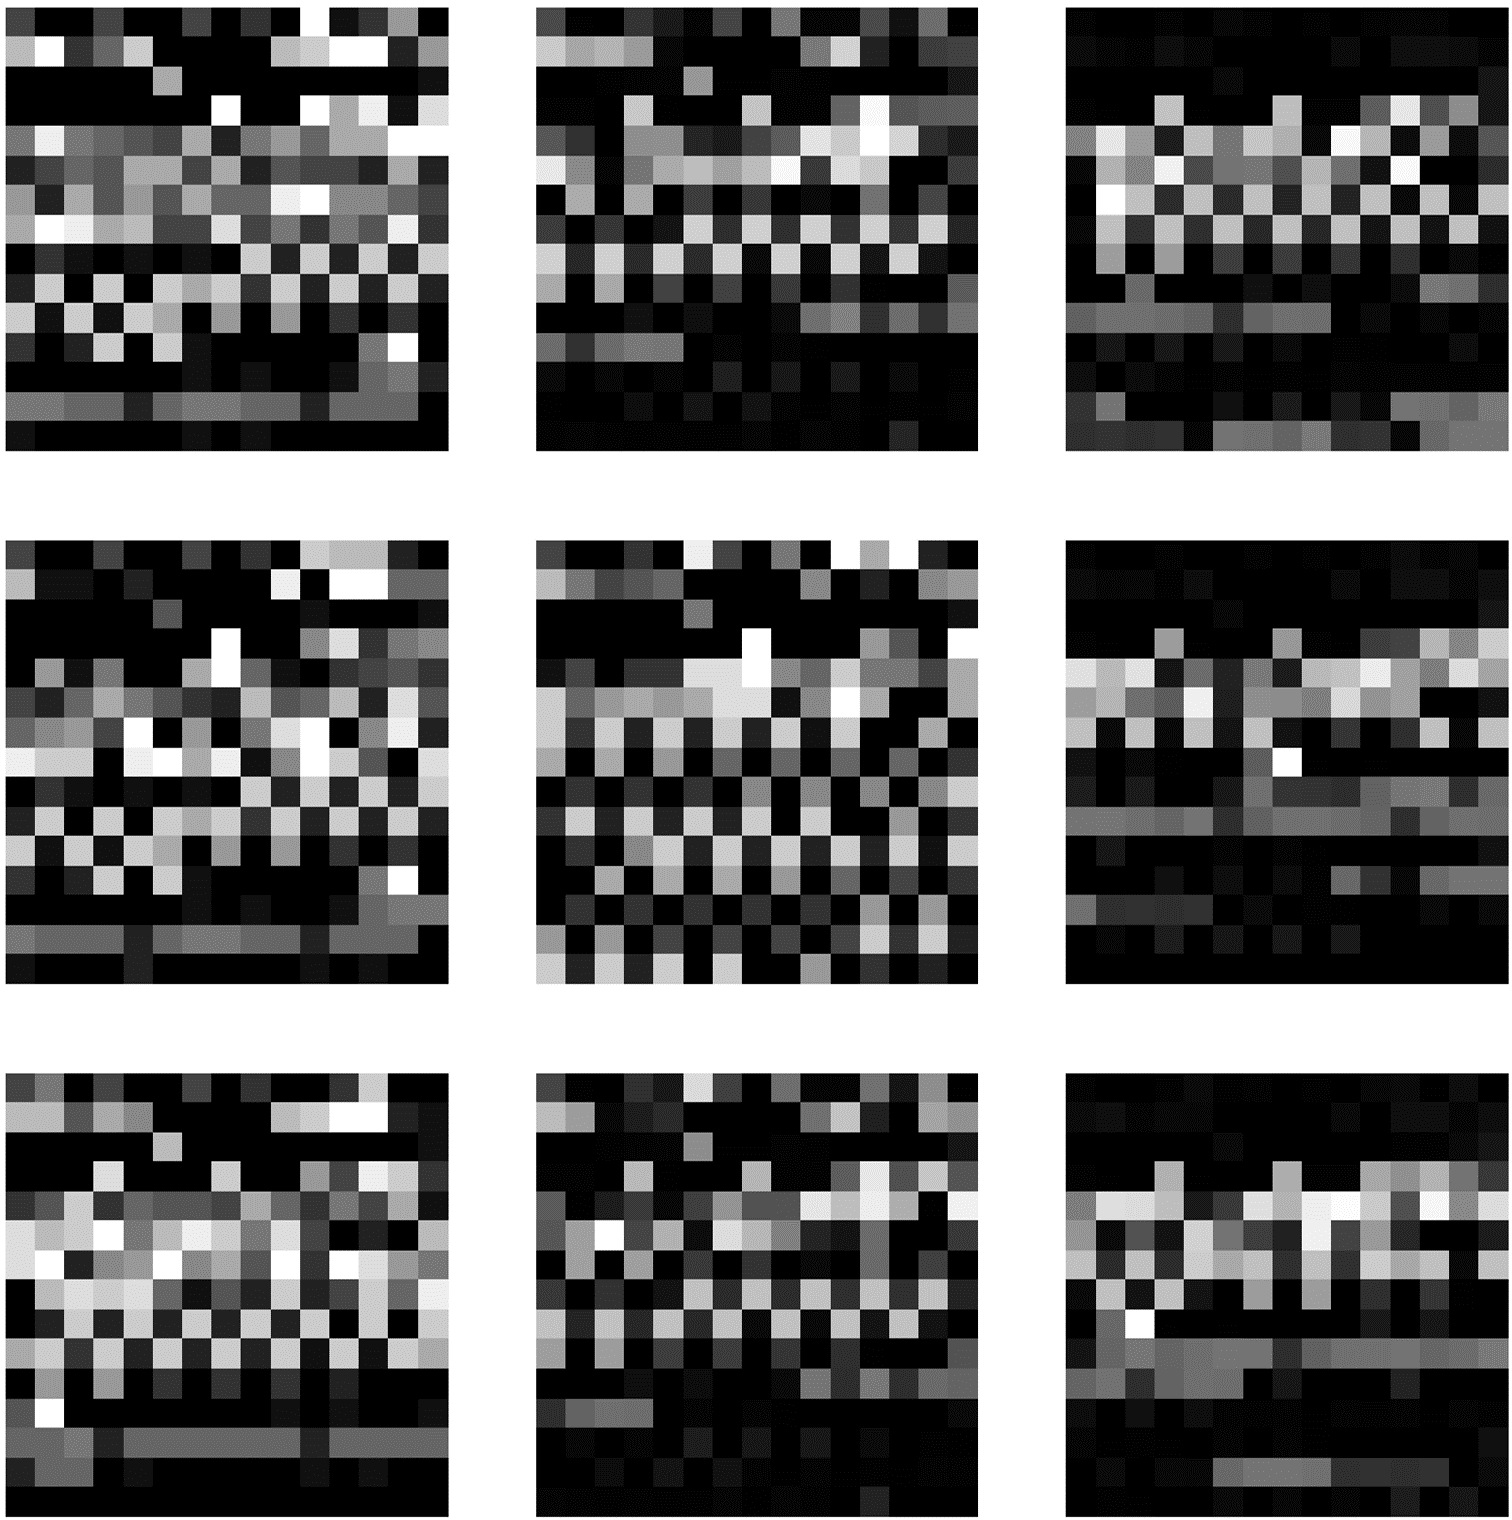
\includegraphics[width=\textwidth]{4-2-1}
      \caption{iOS系统}
    \end{subfigure}%
    \hspace{20pt}
    \begin{subfigure}[b]{0.3\textwidth}
      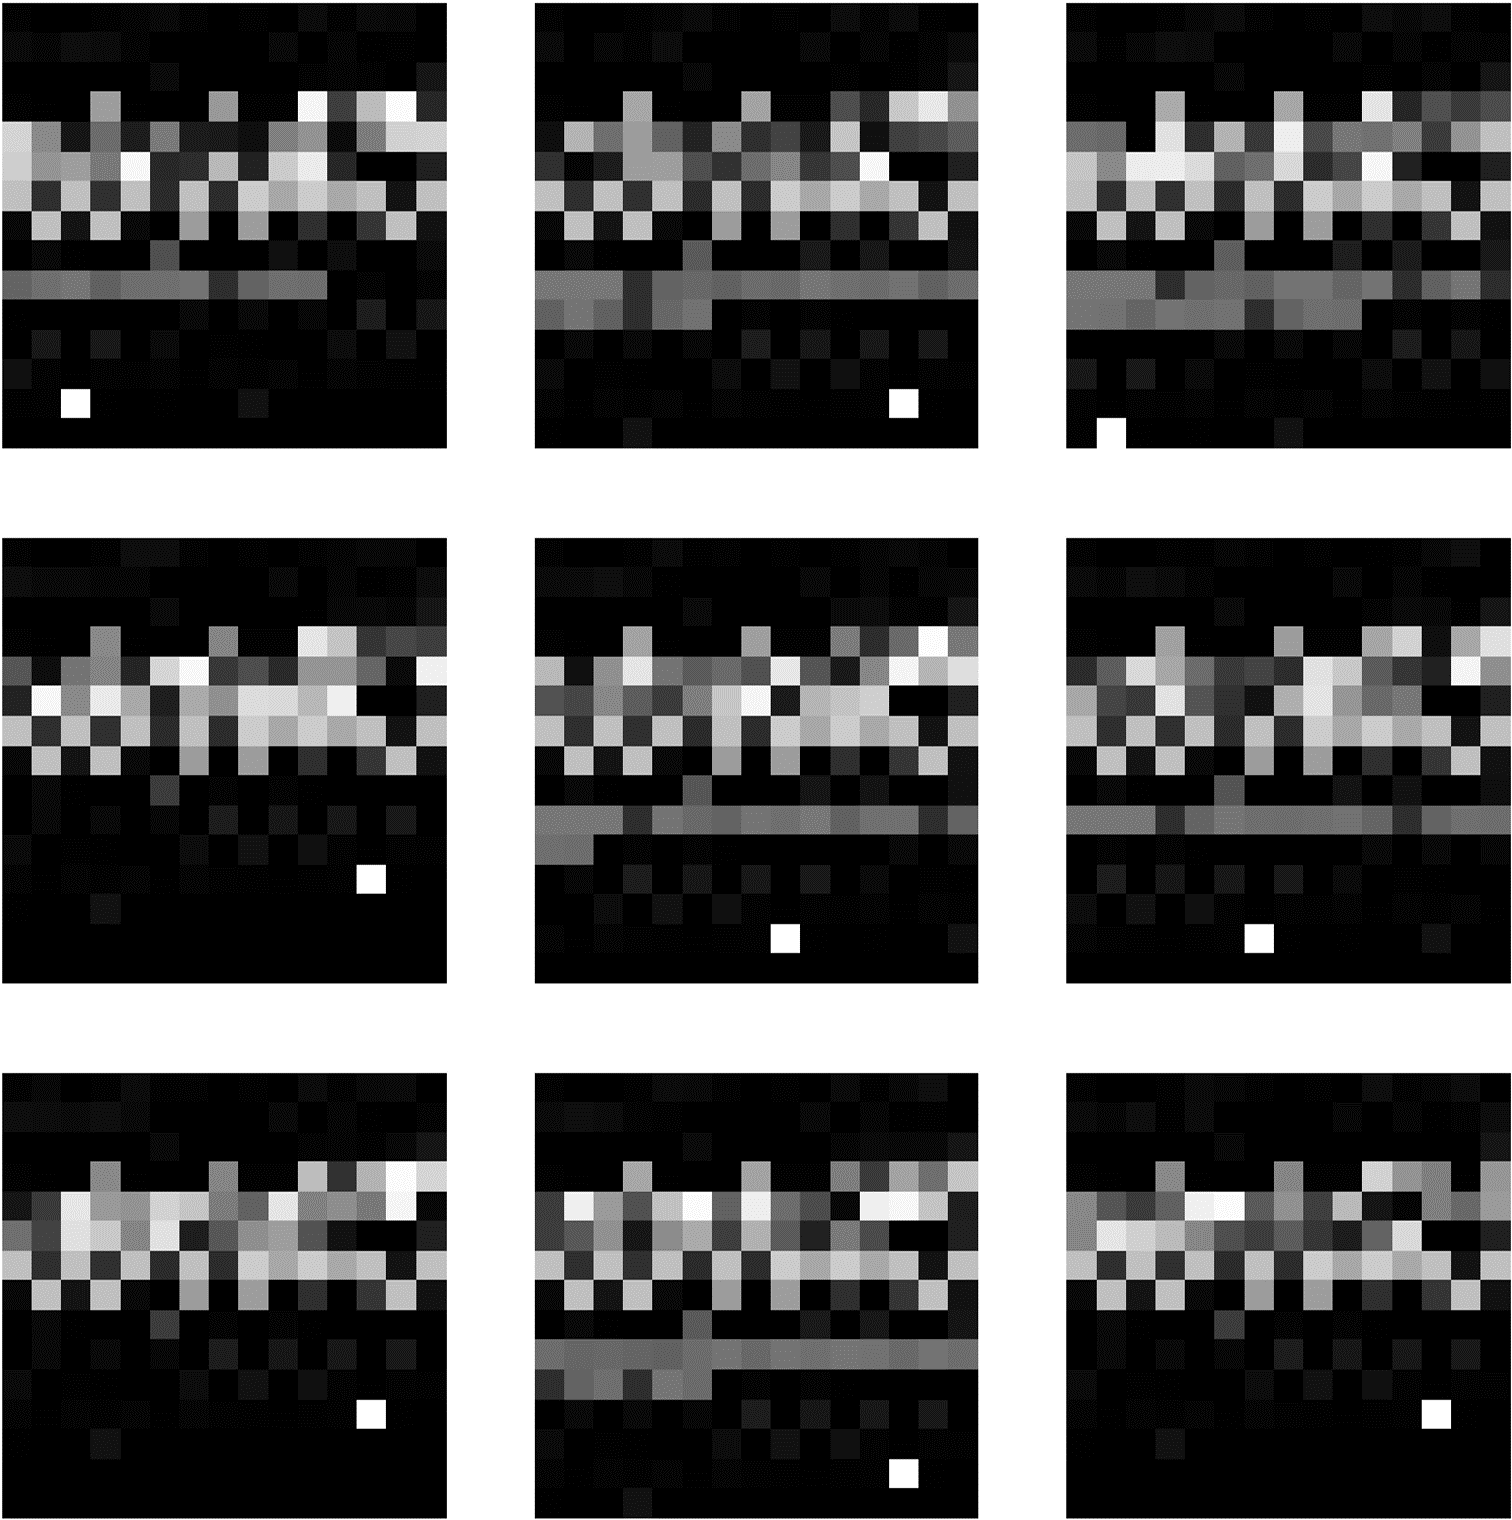
\includegraphics[width=\textwidth]{4-2-2}
      \caption{Linux系统}
    \end{subfigure}
    \bicaption{原始流量灰度图(a)iOS系统,(b)Linux系统}{Gray scale image of raw traffic(a)iOS system, (b)Linux system}
    \label{fig:3-6}
\end{figure}

在控制报文中,可以表达语义信息的最小单位一般是字节(byte),对应的数值为0-255。将TCP SYN包和TLS Client Hello包中的数据拼接后,并绘制256级灰度图,如图4.2所示,分别是由iOS系统和Linux系统产生的九条原始流对应的灰度图。在图a中,可以看到iOS系统发送的多数Client Hello握手报文中都存在高频的大小值交错序列片段,这一现象在其他操作系统的原始流灰度图中是看不到的。在图b中,由Linux系统产生的流量灰度图同样存在可被观察到的一些特征。例如,Client Hello握手报文中的有语义信息主要存在于报文的中上部,并且所有包都在尾部拥有一个独立亮点,其对应数值0xff01,在RFC文档中,该亮点表示TLS协议的重协商信息扩展。

通过对不同操作系统的原始流量可视化分析,可以发现不同属性的主机产生的流量存在显著的局部特征。又因网络流量数据本身所具备的顺序特性,使得主机属性发现技术中的TCP/IP协议栈指纹比较适合利用表征学习算法进行自动挖掘。

\subsection{基于深度前馈神经网络的原始载荷特征挖掘模型}

前馈神经网络是最早发明的简单人工神经网络。在前馈神经网络中,各神经元分别属于不同的层。每一层的神经元可以接收前一层神经元的信号,并产生信号输出到下一层。第一层叫输入层,最后一层叫输出层,其它中间层叫做隐藏层。整个网络中无反馈,信号从输入层向输出层单向传播,可用一个有向无环图表示。前馈神经网络具有很强的拟合能力,常见的连续非线性函数都可以用前馈神经网络来近似。

然而,传统的浅层学习方法受限于小规模的样本和低性能的计算单元,对复杂函数的表示能力有限。深度前馈神经网络(Deep Neural Networks, DNN)通过构建一种深层次的非线性网络结构,从海量训练数据中学习更有用的特征,可以实现复杂函数逼近,展现出了强大的表示学习能力。图4.3给出了只采用全连接层的DNN模型实例。本章构建的DNN网络模型采取5层全连接层作为隐藏层,并将Softmax层作为输出层,如表4.1所示。

\begin{figure}[!htbp]
    \centering
    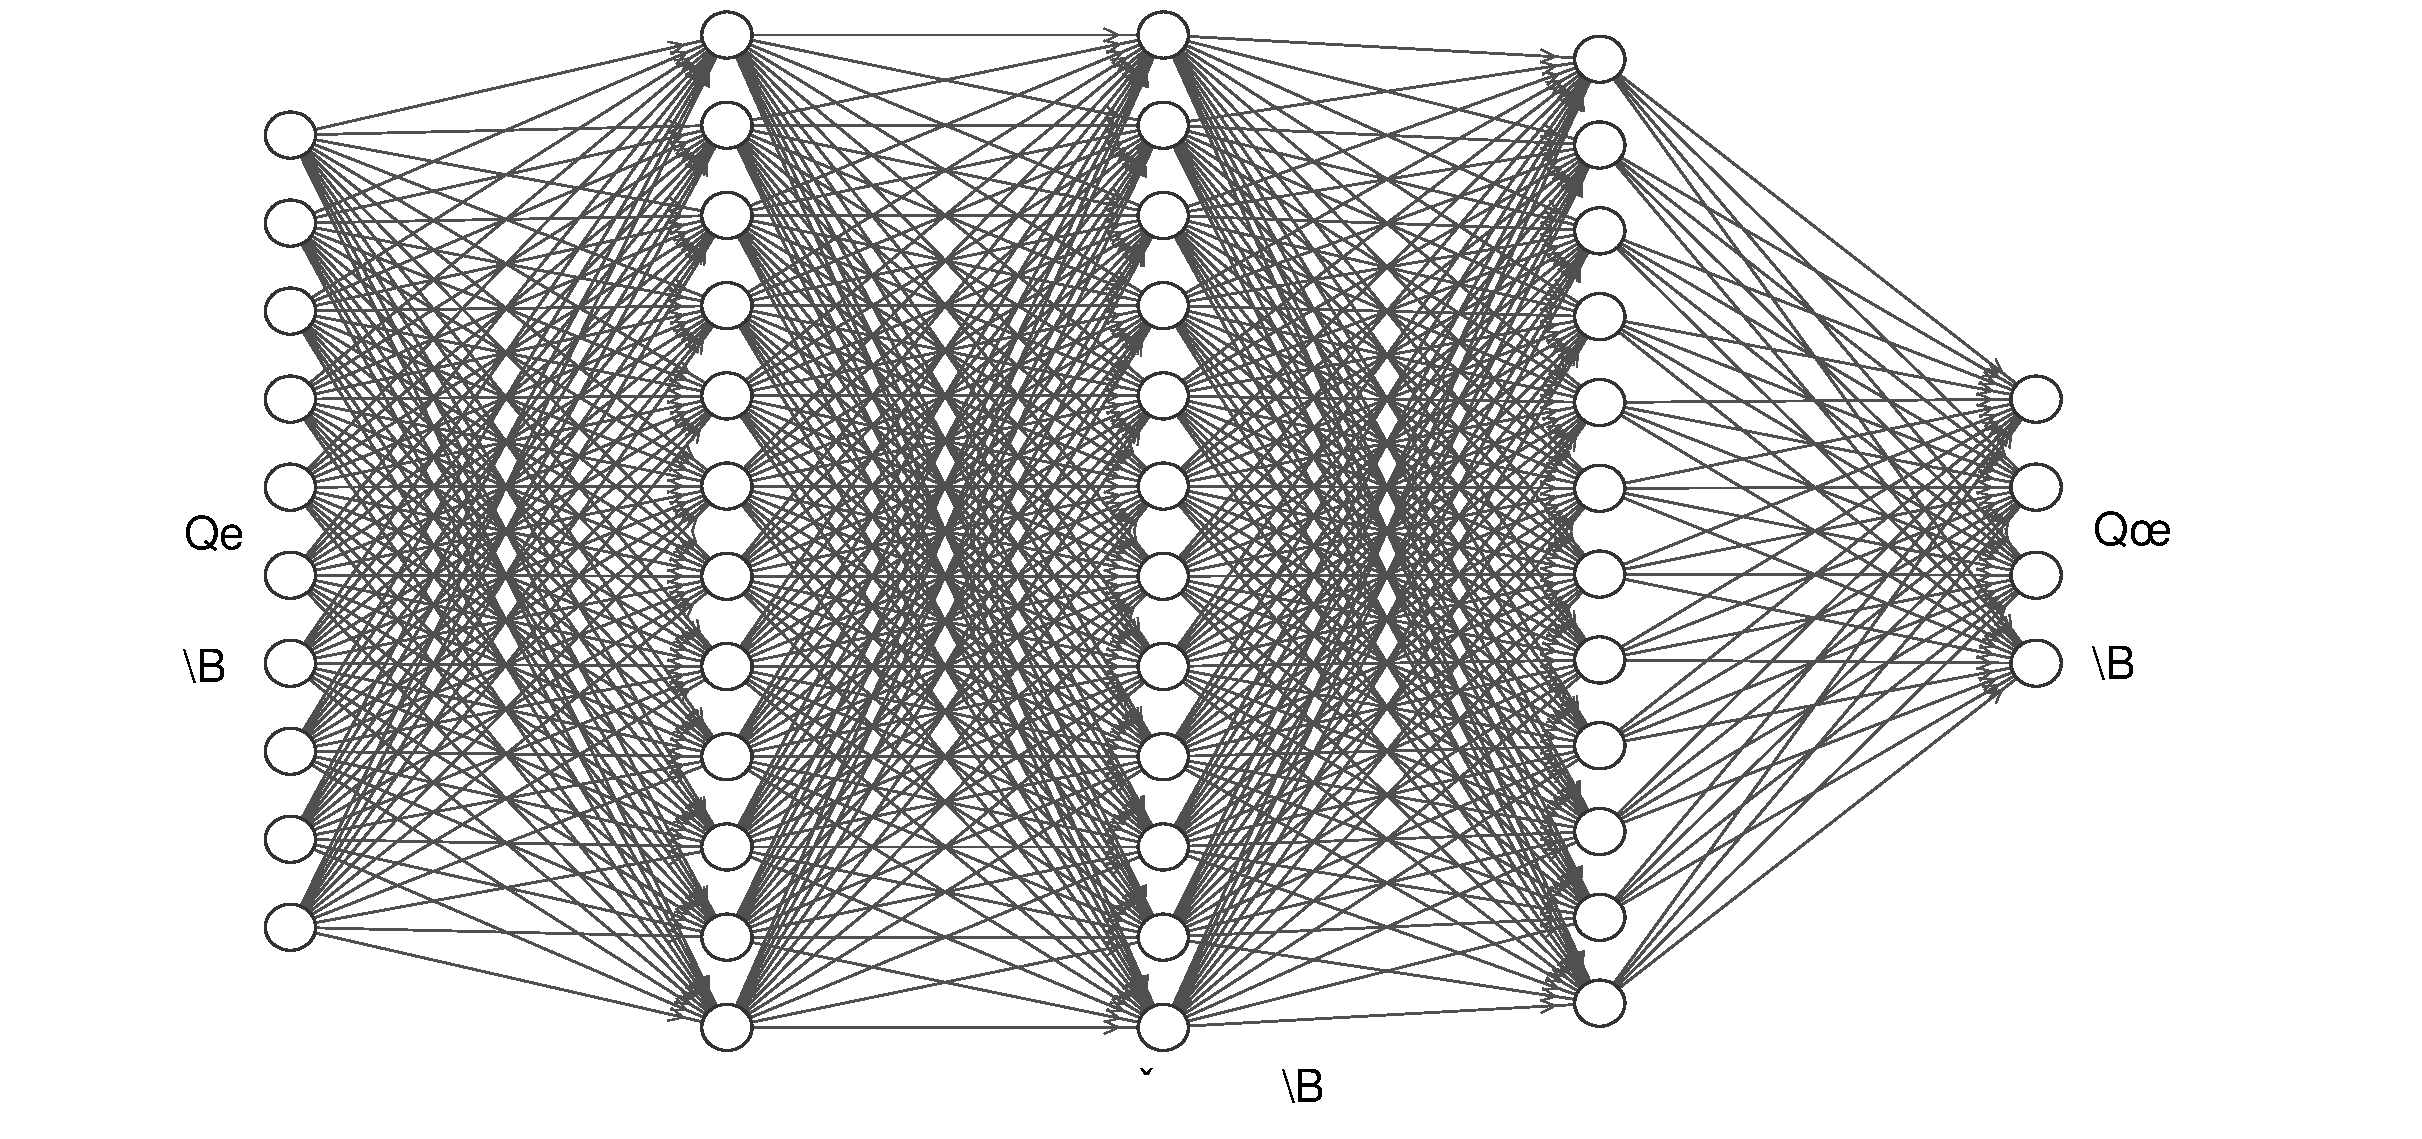
\includegraphics[width=0.9\textwidth]{nn}
    \bicaption{深度全连接网络的一般结构}{General structure of deep fully connected network}
    \label{fig:4-3}
\end{figure}

\begin{table}[!h]
    \bicaption{DNN模型结构参数表}{Structure parameter table of one-dimensional DNN model.}
    \centering
    \footnotesize
    \setlength{\tabcolsep}{15pt}
    \renewcommand{\arraystretch}{1}
\begin{tabular}{cccc}
\toprule
层数&操作&输入维度&输出维度\\
\hline
1 & input & 225 & 512 
\\ 
2 & full connect & 512 & 1024
\\ 
3 & full connect & 1024 & 1024
\\ 
4 & full connect & 1024 & 256
\\ 
5 & full connect & 256 & 128
\\ 
6 & full connect & 128 & 32
\\
7 & softmax & 32 & 5/21
\\ 
\bottomrule
\end{tabular}
\end{table}

\subsection{基于卷积神经网络的原始载荷特征挖掘模型}

%卷积神经网络是一种具有局部连接、权重共享等特性的深层前馈神经网络。卷积神经网络最早是主要用来处理图像信息。如果用全连接前馈网络来处理图像时,会存在参数太多、局部不变性特征等问题。

卷积神经网络是受生物学上感受野的机制启发而提出。感受野(Receptive Field)主要是指听觉、视觉等神经系统中一些神经元的特性,即神经元只接受其所支配的刺激区域内的信号。在视觉神经系统中,视觉皮层中的神经细胞的输出依赖于视网膜上的光感受器。视网膜上的光感受器受刺激兴奋时,将神经冲动信号传到视觉皮层,但不是所有视觉皮层中的神经元都会接受这些信号。一个神经元的感受野是指视网膜上的特定区域,只有这个区域内的刺激才能够激活该神经元。

卷积神经网络有三个结构上的特性:局部连接,权重共享以及汇聚。这些特性使得卷积神经网络具有一定程度上的平移、缩放和旋转不变性。和前馈神经网络相比,卷积神经网络的参数更少。卷积神经网络主要使用在图像和视频分析的各种任务上,比如图像分类、人脸识别、物体识别、图像分割等,其准确率一般也远远超出了其它的神经网络模型。近年来卷积神经网络也广泛地应用到自然语言处理、推荐系统等领域。

\begin{itemize}
\item 局部连接:由于图像的空间联系是局部的,每个神经元不需要对全部的图像做感受,只需要感受局部特征即可,然后在更高层将这些感受得到的不同局部神经元综合起来就可以得到全局信息,达到减少连接的数目。

\item 权重共享:不同神经元之间的参数共享可以减少模型中需要求解的参数,使用多种滤波器对数据进行卷积可以得到多种特征映射。权值共享其实是对数据用同样的卷积核进行卷积操作,使其具备平移不变性。

\end{itemize}

如图4.4所示,一般的卷积神经网络结构包括:卷积层,汇聚层和全连接层。每一层有多个特征图,每个特征图通过一种卷积滤波器提取输入特征,每个特征图有多个神经元。

\begin{figure}[!htbp]
    \centering
    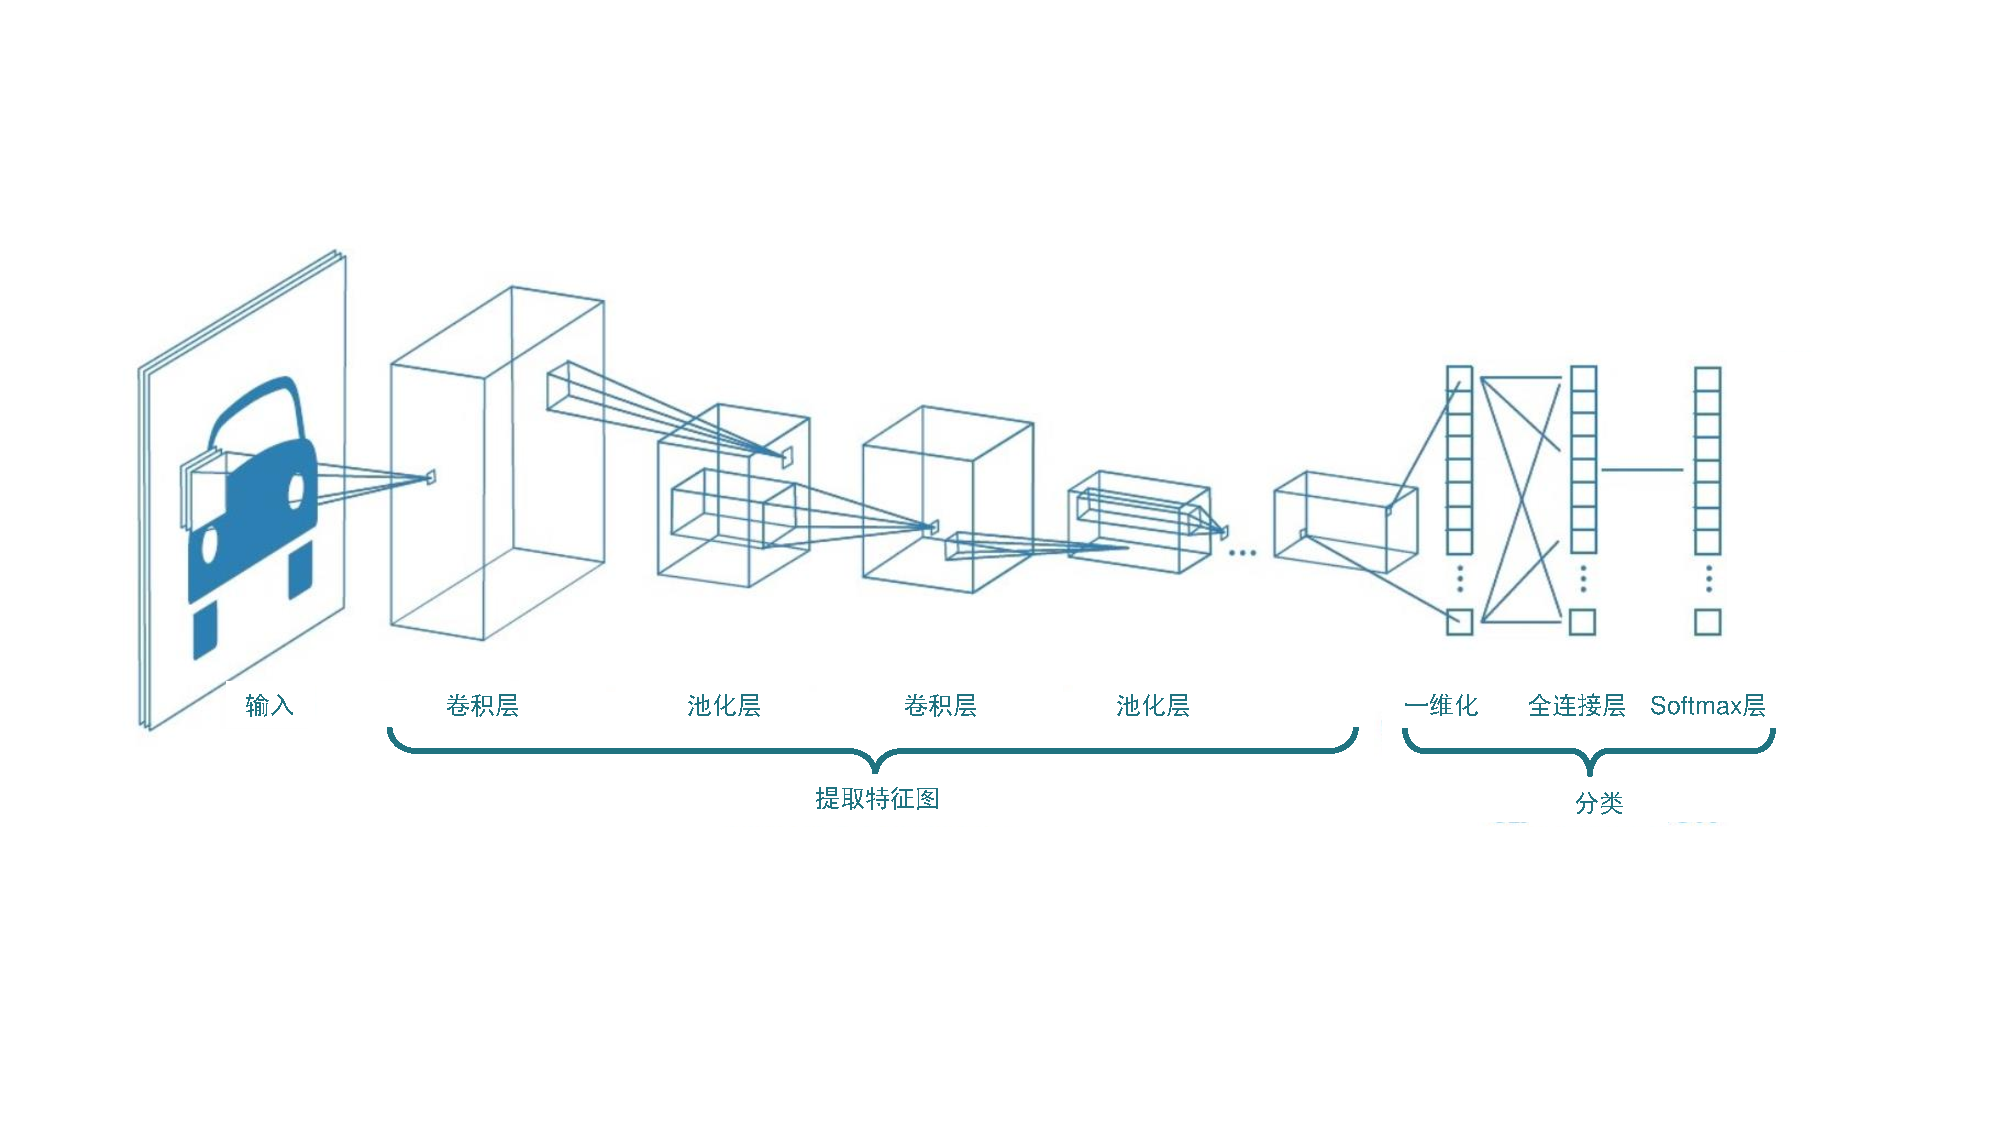
\includegraphics[width=0.8\textwidth]{4-3}
    \bicaption{卷积神经网络的一般结构}{General structure of a convolutional neural network}
    \label{fig:4-3}
\end{figure}

根据所要处理的目标不同,卷积神经网络的常见结构主要分为三种:适合处理序列数据的一维CNN,适合处理图像数据的二维CNN以及适合处理视频数据的三维CNN。在网络流量数据中,报文载荷是一种按层次结构组织的有序一维字节流,其中多个连续字节可组成有一定语义的基础字段,多个连续基础字段又可组成表示特定功能的报文片段,这种有序特性表明网络流数据属于序列数据。因此,本章选择了一维CNN模型作为进行主机属性识别效果实验,同时构建最经典的的二维CNN模型进行对比。

\begin{table}[!h]
    \bicaption{一维CNN模型结构参数表}{Structure parameter table of one-dimensional CNN model}
    \centering
    \footnotesize
    \setlength{\tabcolsep}{8pt}
    \renewcommand{\arraystretch}{1}
\begin{tabular}{ccccccc}
\toprule
层数&操作&输入维度&滤波器&步长&Pad&输出维度\\
\midrule
1 & conv+BN+ReLU & 1@1*225 & 1*3 & 1 & same & 64@1*225 
\\ 
2 & 1d max pool & 64@1*225 & 1*2 & 2 & same & 64@1*113 
\\ 
3 & conv+BN+ReLU & 64@1*113 & 1*3 & 1 & same & 128@1*113
\\ 
4 & 1d max pool &128@1*113 & 1*2 & 2 & same & 128@1*57
\\ 
5 & conv+BN+ReLU & 128@1*57 & 1*3 & 1 & same & 256@1*57
\\ 
6 & conv+BN+ReLU & 256@1*57 & 1*3 & 1 & same & 256@1*57
\\ 
7 & 1d max pool & 256@1*57 & 1*2 & 2 & same & 256@1*29
\\
8 & full connect & 256*29 & -- & -- & none & 1024
\\
9 & full connect & 1024 & -- & -- & none & 5/21
\\ 
10 & softmax & 5/21 & -- & -- & none & 5/21
\\ 
\bottomrule
\end{tabular}
\end{table}

本章构建的一维卷积神经网络模型共包含4层卷积层,3层池化层和2层全连接层,并将Softmax层作为网络的最后一层,最终得到的激活值即为模型识别出的主机属性种类。具体的参数设置如表4.2所示。其中,每层卷积层都选用ReLU函数作为激活函数,并加入了批正则处理。选择ReLU函数可以有效避免深度神经网络的梯度弥散和梯度爆炸问题,而批正则处理可以解决深度网络训练过程中难以收敛的问题,加快训练过程,并在一定程度上缓解过拟合现象。

\begin{table}[!h]
    \bicaption{二维CNN模型结构参数表}{Structure parameter table of two-dimensional CNN model}
    \centering
    \footnotesize
    \setlength{\tabcolsep}{8pt}
    \renewcommand{\arraystretch}{1}
\begin{tabular}{ccccccc}
\toprule
层数&操作&输入维度&滤波器&步长&Pad&输出维度\\
\hline
1 & conv+BN+ReLU & 1@15*15 & 2*2 & 1 & same & 64@15*15 
\\ 
2 & 2d max pool & 64@15*15 & 2*2 & 2 & same & 64@8*8 
\\ 
3 & conv+BN+ReLU & 64@8*8 & 2*2 & 1 & same & 128@8*8
\\ 
4 & conv+BN+ReLU & 128@8*8 & 2*2 & 1 & same & 256@8*8
\\ 
5 & 2d max pool & 256@8*8 & 1*2 & 2 & same & 256@4*4
\\ 
6 & full connect & 256*16 & -- & -- & none & 1024
\\ 
7 & full connect & 1024 & -- & -- & none & 5/21
\\ 
8 & softmax & 5/21 & -- & -- & none & 5/21
\\ 
\bottomrule
\end{tabular}
\end{table}

如表4.3所示,二维卷积神经网络模型主要包含3层卷积层,2层池化层和2层全连接层。同一维CNN卷积神经网络模型,每层卷积层都选用ReLU函数作为激活函数,并加入批正则处理。

\subsection{基于长短期记忆网络的原始载荷特征挖掘模型}

循环神经网络是一类具有短期记忆能力的神经网络。在循环神经网络中,神经元不但可以接受其它神经元的信息,也可以接受自身的信息,形成具有环路的网络结构。和前馈神经网络相比,循环神经网络更加符合生物神经网络的结构。循环神经网络已经被广泛应用在语音识别、语言模型以及自然语言生成等任务上。循环神经网络的参数学习可以通过随时间反向传播算法来学习。随时间反向传播算法即按照时间的逆序将错误信息一步步地往前传递。当输入序列比较长时,会存在梯度爆炸和消失问题,也称为长程依赖问题。

为了改善循环神经网络的长程依赖问题,目前最有效的改进方式就是通过引入门控机制来控制信息的累积速度,包括有选择地加入新的信息,并有选择地遗忘之前累积的信息。这一类网络可以称为基于门控的循环神经网络,最流行的代表就是长短期记忆(LSTM)网络。如图4.5所示,LSTM网络主要通过三种门实现门控机制:遗忘门、输入门和输出门。

\begin{itemize}
\item 遗忘门:控制上一个时刻的内部状态需要遗忘多少信息。
\item 输入门:控制当前时刻的输入有多少信息需要保存。
\item 输出门:控制当前时刻的内部状态有多少信息需要输出给外部状态。 
\end{itemize}

\begin{figure}[!htbp]
    \centering
    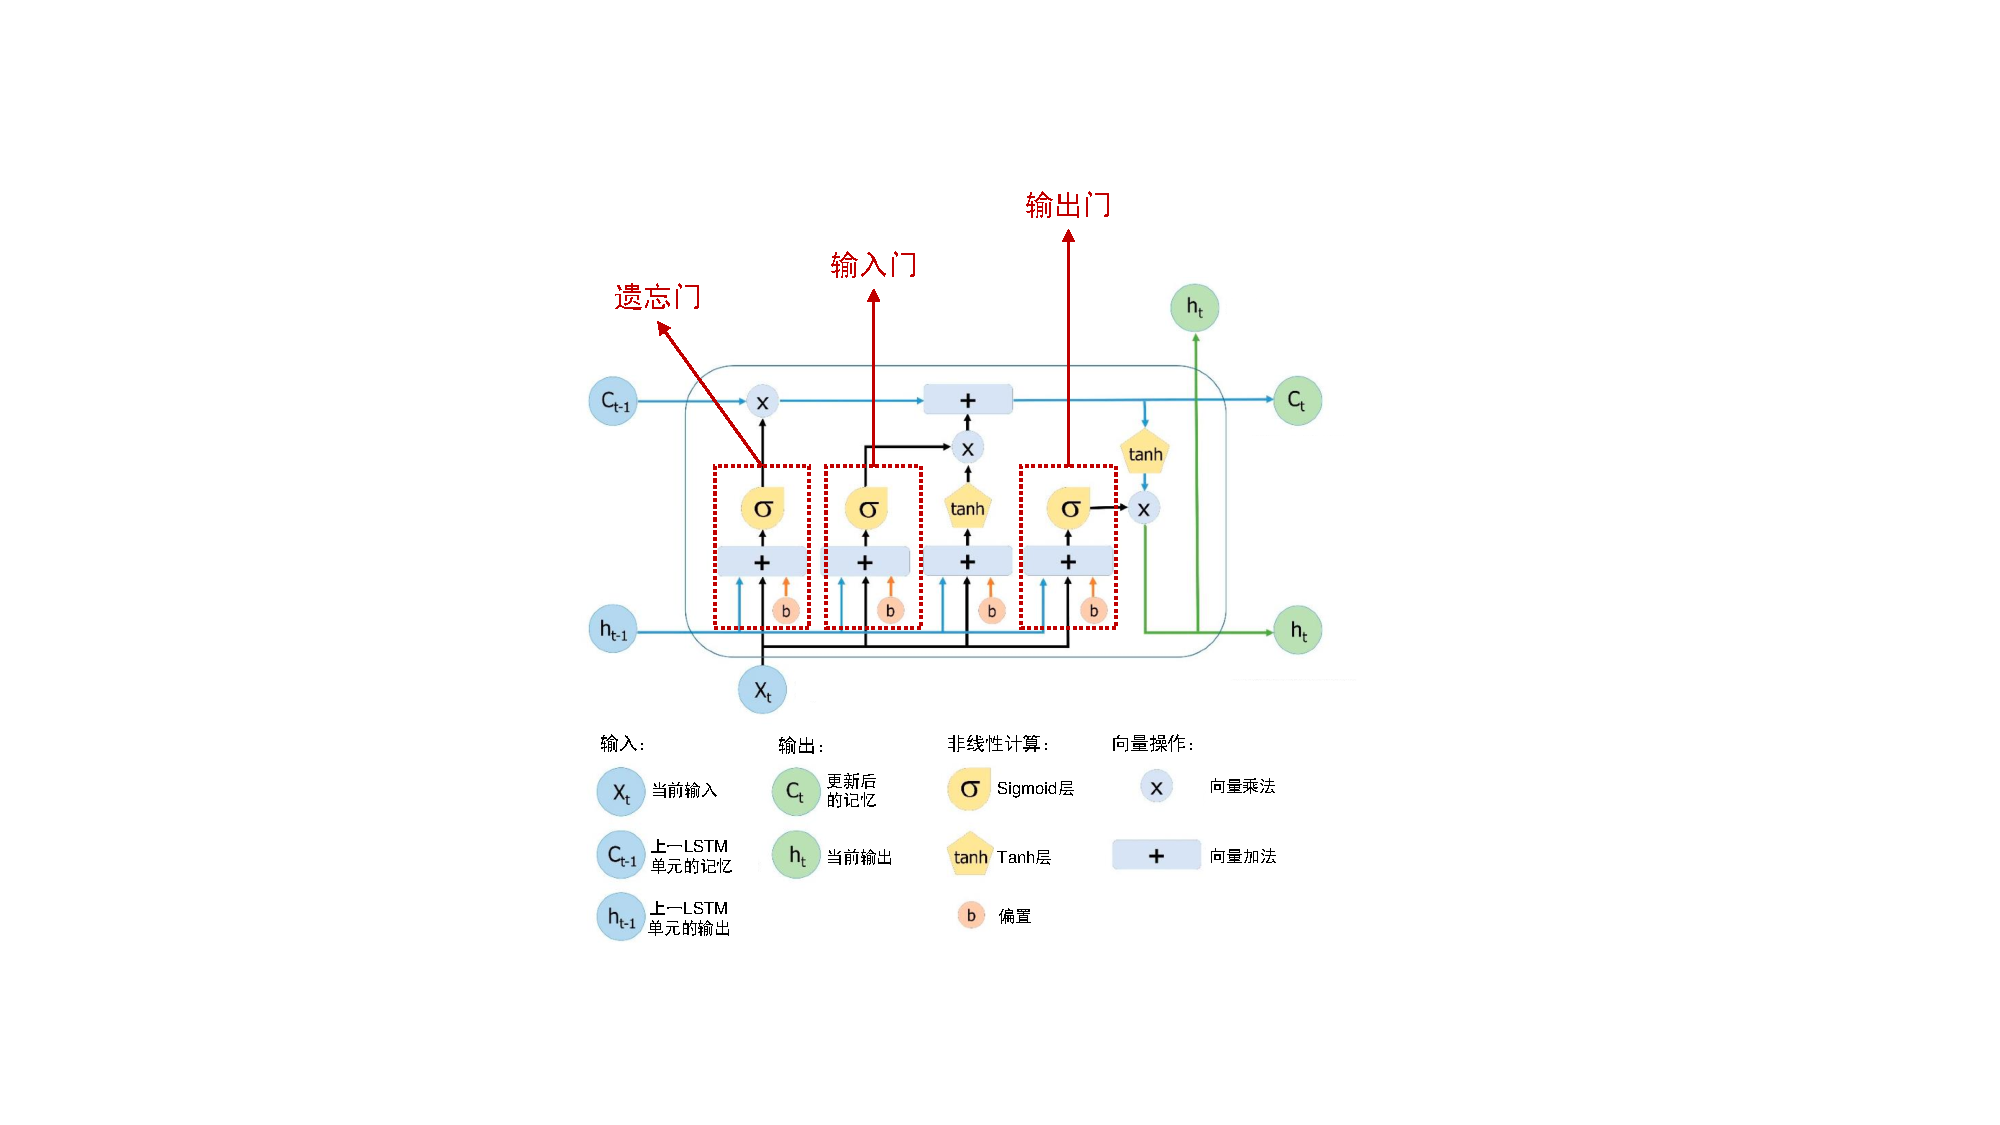
\includegraphics[width=0.7\textwidth]{4-4}
    \bicaption{LSTM网络的一般结构}{General structure of LSTM network}
    \label{fig:4-4}
\end{figure}

本章构建了一个单层LSTM网络模型,结合交叉验证法和超参数网格搜索得到的最佳模型参数如表4.4所示。其中,序列段长度为4,隐藏层节点数目为256,遗忘因子为0.1,并在输入位置添加了Dropout处理,避免过拟合问题的出现,提高模型在测试集上的性能。

\begin{table}[!htbp] 
    \bicaption{LSTM模型结构参数表}{Structure parameter table of two-dimensional LSTM model}
%    \label{tab:sample}
    \centering
    \footnotesize
    \setlength{\tabcolsep}{25pt}
    \renewcommand{\arraystretch}{1}
\begin{tabular}{lll}
\toprule
参数 & 含义 & 取值 \\ \hline
time\underline{~~}step & 序列段长度 & 4 \\ 
rnn\underline{~~}unit & 隐藏层节点数 & 256 \\ 
forget\underline{~~}bias & 遗忘因子 & 0.1 \\ 
\bottomrule
\end{tabular}
\end{table}

\subsection{模型效果对比}

为了选择适合主机属性发现任务的最佳深度学习模型,本节从分类准确率、精度、召回率以及PR曲线等角度对深度全连接网络、一维卷积神经网络、二维卷积神经网络以及长短期记忆网络等模型进行效果对比实验。同时,为了展示基于加密流原始载荷的主机属性方法的优越性,引入第三章中基于人工特征的最优模型即LightGBM模型共同进行对比实验。本节实验均采用Tensorflow框架来实现各种深度学习模型,其他实验环境参数详情以及数据集详情参照3.4节和3.5节。

\begin{figure}[!h]
    \centering
    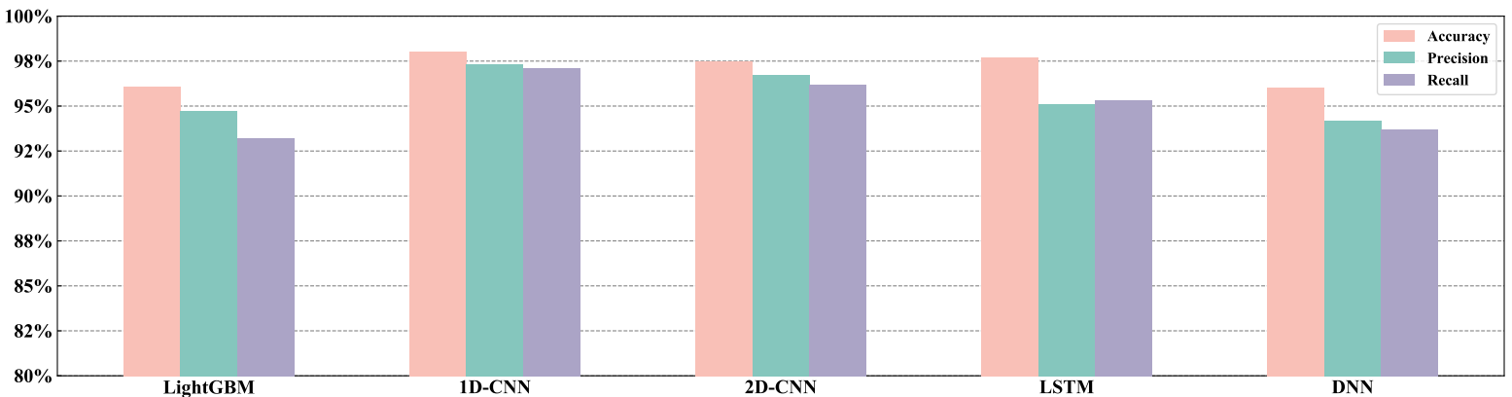
\includegraphics[width=0.9\textwidth]{4-5}
    \bicaption{模型准确率、精度和召回率对比}{Comparison of model accuracy, precision and recall}
    \label{fig:4-4}
\end{figure}

\begin{figure}[!h]
    \centering
    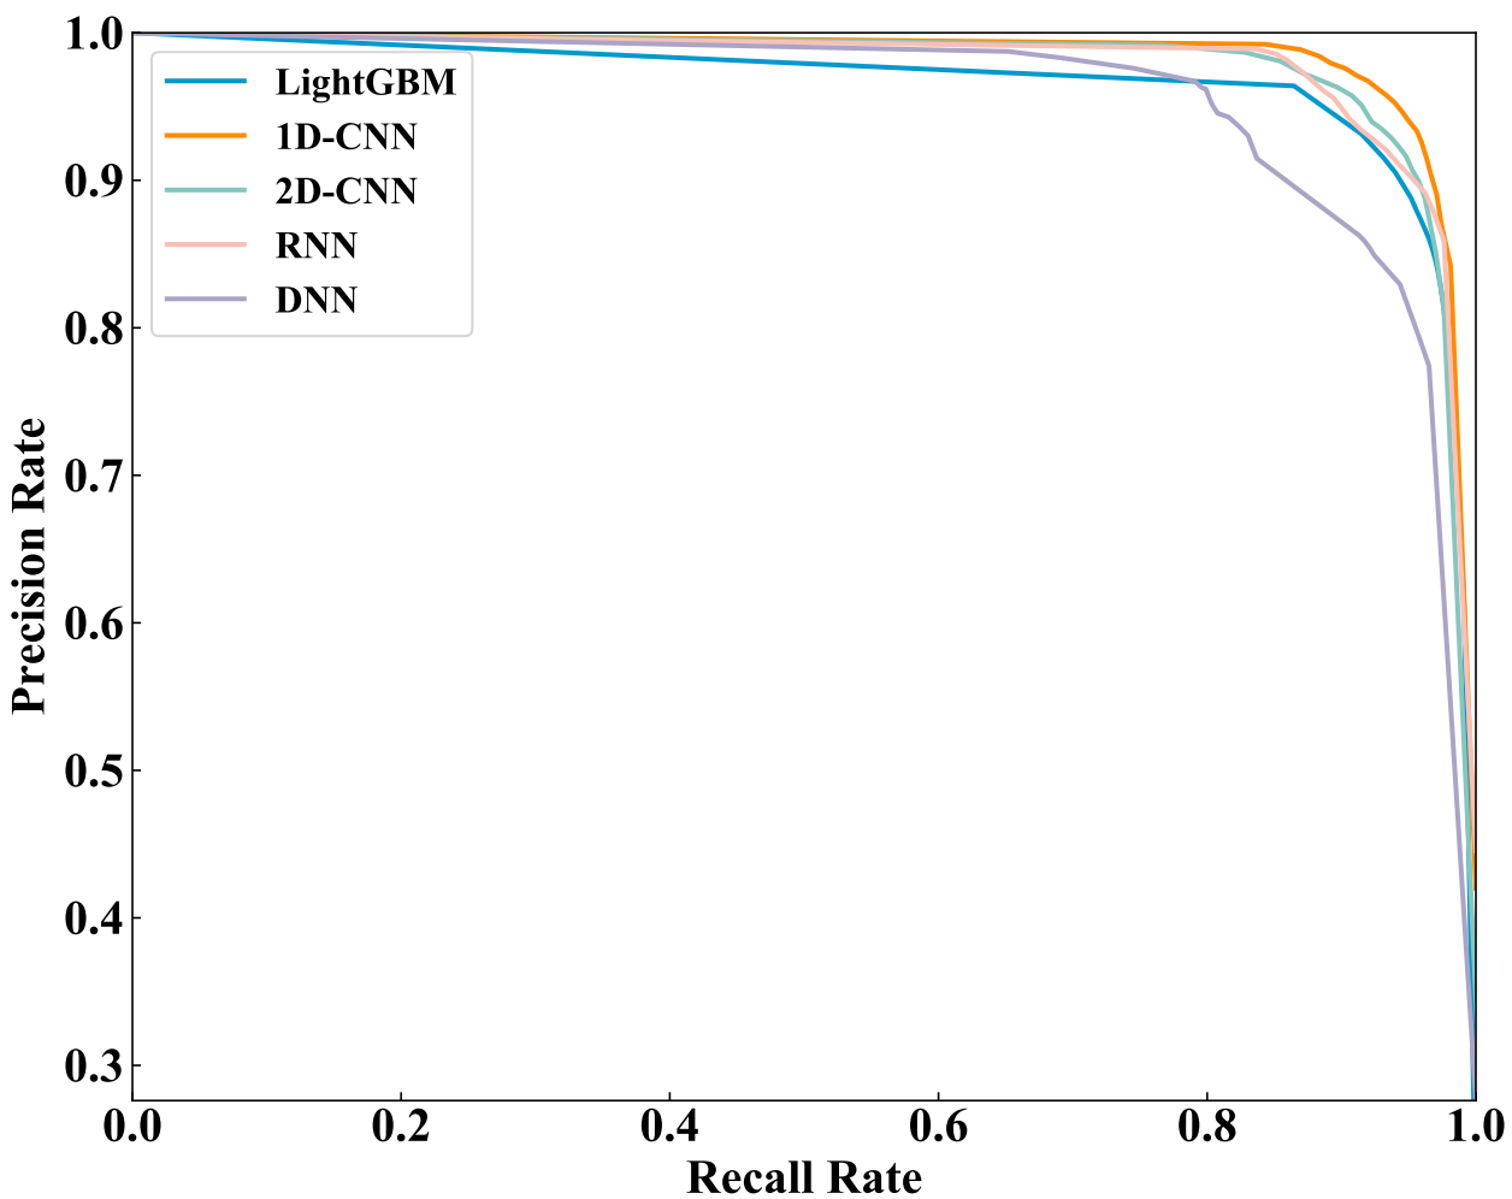
\includegraphics[width=0.6\textwidth]{4-6}
    \bicaption{模型PR曲线对比}{Model PR curve comparison}
    \label{fig:4-4}
\end{figure}

如图4.6和4.7所示,从准确率、精度、召回率和PR曲线等评估指标来看,一维CNN模型在众多神经网络模型中有着最佳表现。而且和从人工特征数据集中训练出的LightGBM模型相比,一维CNN模型的准确率、精度和召回率都提高了近3\%,PR曲线也完全包住了LightGBM模型的PR曲线。以上实验结果都证明一维CNN模型是最适合主机属性发现任务的神经网络模型。



\section{基于加密流原始载荷的主机属性发现结果}

基于加密流原始载荷的主机属性发现技术以一维卷积神经网络作为分类器,将TCP SYN包和TLS Clinet Hello包的原始流信息经过数据归一化处理后作为输入,便可识别目标主机的各种属性。

将数据集按照日期进行切分,以前四天的数据作为训练集,以最后一天的数据作为测试集,可得到如表4.5-4.7的识别结果。

\begin{table}[!h]
    \bicaption{操作系统类型识别结果}{Operating system type identification results}
    \centering
    \footnotesize
    \setlength{\tabcolsep}{8pt}
    \renewcommand{\arraystretch}{1}
\begin{tabular}{|c|c|c|c|c|c|c|c|}
\hline
\multirow{2}{*}{ \textbf{ID}} & \multirow{2}{*}{ \textbf{操作系统类型}} & \multicolumn{3}{c|}{ \textbf{训练集}} & \multicolumn{3}{c|}{ \textbf{测试集}} \\ \cline{3-8} 
 &  &  \textbf{Precision} &  \textbf{Recall} &  \textbf{F1} & \textbf{Precision} &  \textbf{Recall} &  \textbf{F1} \\ \hline
1 & Android & 98.10\% & 98.07\% & 98.08\% & 97.86\% & 97.85\% & 97.86\% \\ \hline
2 & iOS & 77.29\% & 75.88\% & 76.58\% & 74.15\% & 70.82\% & 72.45\% \\ \hline
3 & Windows & 97.87\% & 98.23\% & 98.05\% & 97.54\% & 97.95\% & 97.74\% \\ \hline
4 & MacOS & 99.21\% & 97.61\% & 98.40\% & 99.03\% & 97.79\% & 98.40\% \\ \hline
5 & Linux & 99.64\% & 99.25\% & 99.44\% & 99.37\% & 98.84\% & 99.10\% \\ \hline
\multicolumn{2}{|c|}{\textbf{AVE}} & 94.42\% & 93.81\% & 94.11\% & 93.59\% & 92.65\% & 93.11\%\\ \hline
\multicolumn{2}{|c|}{\textbf{Accuracy}} & \multicolumn{3}{c|}{98.79\%} & \multicolumn{3}{c|}{98.17\%} \\ \hline
\end{tabular}
\end{table}

在操作系统类型识别任务中,Linux系统的识别效果最好,精度为99.37\%,召回率为98.84\%,F1分数为99.10\%,远高于平均值。由在4.2节中分析的Linux系统原始流量灰度图可知,其TLS协议中存在一个区分度非常高的重协商信息扩展,使得Linux系统的样本容易被分类器识别。iOS系统的识别效果最差,F1分数仅有72.45\%,可能是因为iOS系统原始流量的局部特征不够明显导致。

\begin{table}[!h]
    \bicaption{操作系统版本识别结果}{Operating system version identification results}
    \centering
    \footnotesize
    \setlength{\tabcolsep}{8pt}
    \renewcommand{\arraystretch}{1}
\begin{tabular}{|c|c|c|c|c|c|c|c|}
\hline
\multirow{2}{*}{\textbf{ID}} & \multirow{2}{*}{\textbf{操作系统版本}}  & \multicolumn{2}{c|}{\textbf{测试集}} & \multirow{2}{*}{\textbf{ID}} & \multirow{2}{*}{\textbf{操作系统版本}}  & \multicolumn{2}{c|}{\textbf{测试集}} \\ \cline{3-4} \cline{7-8}
 &  & \textbf{Precision} & \textbf{Recall}  & & & \textbf{Precision} & \textbf{Recall} \\ \hline
1 & Android 4 & 78.99\% & 61.58\% &12 & iOS 7 & 98.86\% & 98.86\% \\ \hline
2 & Android 5 & 83.90\% & 74.63\% &13 & iOS 8 & 36.36\% & 30.77\% \\ \hline
3 & Android 6 & 88.21\% & 77.85\% &14 & iOS 9 & 80.30\% & 77.94\% \\ \hline
4 & Android 7 & 92.18\% & 62.48\% &15 & iOS 10 & 61.54\% & 53.33\% \\ \hline
5 & Android 8 & 63.68\% & 78.11\% &16 & iOS 11 & 77.01\% & 80.72\% \\ \hline
6 & Android 9 & 66.73\% & 72.05\% &17 & iOS 12 & 40.06\% & 66.83\% \\ \hline
7 & Windows XP & 85.40\% & 76.35\% &18 & MacOS 10 & 98.87\% & 99.15\% \\ \hline
8 & Windows 7 & 92.41\% & 92.96\% &19 & MacOS 11 & 99.63\% & 99.57\% \\ \hline
9 & Windows 8 & 100.00\% & 36.59\% &20 & MacOS 12 & 98.61\% & 91.03\% \\ \hline
10 & Windows 8.1 & 97.30\% & 80.45\% &21 & Ubuntu & 99.51\% & 99.12\% \\ \hline
11 & Windows 10 & 95.94\% & 97.66\% & \multicolumn{2}{c|}{\textbf{AVE}}& 78.78\% & 73.04\% \\ \hline
\end{tabular}
\end{table}

在操作系统版本识别任务中,总体识别效果要明显差于操作系统类型识别任务结果,这是因为操作系统版本识别任务是一个细粒度主机属性识别任务,本质上是一个21类分类任务,而操作系统类型识别任务是一个5类分类任务。一般而言,对于同等规模的训练数据集,深度学习模型的预测能力与预测类别数目成反比。在具体识别结果中,Windows8系统的识别精度为100\%,召回率却只有36.59\%,精度和召回率相差十分明显的原因主要有两个,一个是Windows 8的样本量在数据集中的比例较小,第二个原因是Windows 8和Windows 8.1的网络协议栈实现差异性较小,在协议指纹上的区分度不明显,导致了其识别召回率非常差。同样的问题也存在于部分iOS系统的版本识别结果中。

\begin{table}[!h]
    \bicaption{浏览器类型识别结果}{Browser type identification results}
    \centering
    \footnotesize
    \setlength{\tabcolsep}{8pt}
    \renewcommand{\arraystretch}{1}
\begin{tabular}{|c|c|c|c|c|c|c|c|}
\hline
\multirow{2}{*}{ \textbf{ID}} & \multirow{2}{*}{ \textbf{浏览器类型}} & \multicolumn{3}{c|}{ \textbf{训练集}} & \multicolumn{3}{c|}{ \textbf{测试集}} \\ \cline{3-8} 
 &  &  \textbf{Precision} &  \textbf{Recall} &  \textbf{F1} & \textbf{Precision} &  \textbf{Recall} &  \textbf{F1} \\ \hline
1 & Firefox & 97.90\% & 88.50\% & 92.96\% & 97.12\% & 86.33\% & 91.41\% \\ \hline
2 & Safari & 94.72\% & 88.76\% & 91.64\% & 94.32\% & 85.79\% & 89.85\% \\ \hline
3 & Chrome & 97.68\% & 99.52\% & 98.59\% & 97.42\% & 99.43\% & 98.41\% \\ \hline
4 & IE & 94.66\% & 77.24\% & 85.07\% & 92.91\% & 75.78\% & 83.48\% \\ \hline
5 & Opera & 91.37\% & 89.70\% & 90.13\% & 95.81\% & 87.47\% & 90.66\% \\ \hline
\multicolumn{2}{|c|}{\textbf{AVE}} & 95.27\% & 88.74\% & 91.68\% & 95.52\% & 86.96\% & 90.76\%\\ \hline
\multicolumn{2}{|c|}{\textbf{Accuracy}} & \multicolumn{3}{c|}{97.43\%} & \multicolumn{3}{c|}{97.10\%} \\ \hline
\end{tabular}
\end{table}

在浏览器类型识别任务中,Chrome浏览器的识别效果最佳,精度为97.42\%,召回率为99.43\%,F1分数为98.41\%。相对于利用人工提取特征的机器学习模型,神经网络模型对于Chrome浏览器的识别精度明显提升,充分体现了表示学习的优越性。IE浏览器的识别效果相对较差,F1分数为83.48\%,可能是由于其原始字节序列中的局部特征较少。

\section{本章小结}

本章介绍了基于加密流原始载荷的主机属性发现技术,利用表示学习的思想,不需要任何专家知识,只需将网络流的原始流数据作为分类器输入,便可完成细粒度的主机属性发现,并拥有相对于传统方法更佳的识别效果。对于各种流行的深度学习模型,通过分组实验对比在主机属性识别任务中的各类评估指标,发现一维卷积神经网络的适应性最佳。在识别任务的实验结果中,该技术在准确率、精度、召回率以及F1值等方面,效果均优于基于TCP/IP协议栈指纹的LightGBM模型。


